
\section{Minding the Gap}
\label{sec:evaluation}

If achievable, coordination-freedom enables scalability limited to
that of available hardware: namely, server and network capacity. This
is powerful: a \cfree application can scale out without sacrificing
correctness, latency, or availability. In
Section~\ref{sec:bcc-practice}, we saw how many combinations of
invariants and transactions were not \iconfluent and how others were
not; in this section, we examine the implications of these results.

We begin by looking at the real-world costs of coordination: what
happens if \iconfluence does not hold? We quantify upper bounds on
throughput under common network delays. We next examine several
applications to understand whether their transactions are
implementable in a \cfree manner. We first focus on the current
standard for transactional performance---the TPC-C benchmark---and
show---both via \iconfluence analysis and by linearly scaling a
proof-of-concept implementation on public cloud infrastructure---that,
in contrast with classic, coordination-intensive execution strategies,
it is indeed achievable without distributed coordination. We next
examine several other benchmarks as recently proposed in the
literature and discuss their significance with respect to \cfreedom in
real world deployments.

\subsection{Costs of Coordination}

\begin{figure}
  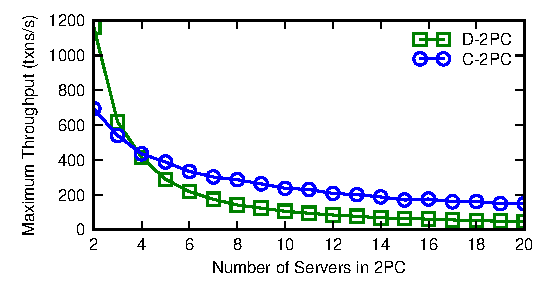
\includegraphics[width=\columnwidth]{figs/singledc-twopc.pdf}\\ {\centering
    \textbf{\scriptsize a.) Local-area network scenario based on
      traces from~\cite{bobtail}}\par}
  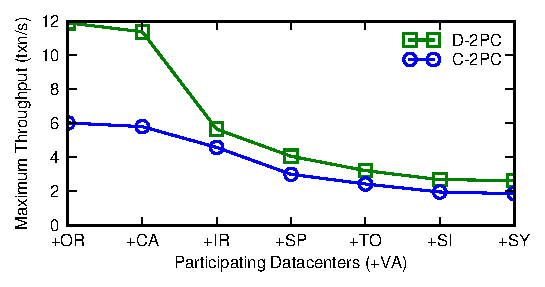
\includegraphics[width=\columnwidth]{figs/multidc-twopc.pdf}\\ \textbf{\scriptsize
    b.) Wide-area network scenario based on traces
    from~\cite{hat-vldb} with transactions originating from a
    coordinator in VA (VA:~Virginia, OR:~Oregon, CA:~California,
    IR:~Ireland, SP:~S\~{a}o Paulo, TO:~Tokyo, SI:~Singapore,
    SY:~Sydney)}

\caption{Atomic commitment latency as an upper bound on throughput
  over LAN and WAN networks.}
\label{fig:2pc}
\end{figure}

What happens if a system must coordinate? One of the primary
challenges in scaling non-\cfree transactions is the atomic commitment
problem: if a transaction might abort, all servers it accesses
(whether replicas of the same item or replicas of different items)
must agree to unilaterally commit or abort the
transaction~\cite{bernstein-book}. For example, in a serializable
database system, a system might check for read-write conflicts and
abort a transaction if any are found. In a coordination-avoiding
system, a system will have to check that non-\iconfluent transactions
do not violate a given invariant (i.e., requiring mutual
exclusion). This \textit{atomic commitment} problem is well studied in
both the database and distributed systems literature, with many
variants~\cite{atomictransactions,paxos-commit,traiger-tods} and poses
a scalability limitation because its latency limits
throughput. Multiple commitment rounds can often proceed in parallel
(e.g., any two \iconfluent transactions can independently commit),
but, at the granularity of a single record (i.e., a worst-case
scenario), atomic commitment becomes a bottleneck. There are many
possible optimizations including batching of commits~\cite{calvin},
but, for arbitrary schedules of transactions, atomic commitment
induces an upper bound on per-item throughput for conflicting
operations.

We performed a simple analysis using recently published datasets of
real-world communication delay from both local-area~\cite{bobtail} and
wide-area~\cite{hat-vldb} networks. We used Monte Carlo analysis to
simulate both traditional two-phase commit (using a coordinator, two
delays of $N$ messages each)~\cite{bernstein-book} (\cpc) and
decentralized two-phase commit (without a coordinator, one delay of
$N^2$ messages)~\cite{paxos-commit} (\dpc), assuming perfect
pipelining (i.e., send \texttt{prepared} immediately after
\texttt{commit}, with no aborts) and only considering network latency
(i.e., local processing time due to locking, latching, validation, or
I/O delays would only increase latency).

Figure~\ref{fig:2pc} show our results for both local-area
(\ref{fig:2pc}a) and wide-area (\ref{fig:2pc}b) networks.  In the
local area, with only two servers participating in atomic commitment
(e.g., replication factor of $2$ or, alternatively, two conflicting
operations on items residing on different servers), we see a maximum
attainable throughput of approximately $1100$ transactions per second
(via \dpc; $750$/s via \cpc). With ten servers participating, \dpc
throughput drops to only $120$ transactions per second (resp. $200$
for \cpc): the long tail of network latency surfaces as the number of
messages sent increases. In the wide area, the effects are stark: if
only coordinating within the continental US from Virginia to Oregon,
\dpc message delays incur a latency of approximately $83$~ms per
commit, resulting in a throughput of $12$ operations per second. If
coordinating between all eight EC2 availability zones, throughput
drops to slightly over $2$ transactions per second in both algorithms.

While this study is based solely on reported latencies, deployment
reports corroborate our findings. For example, Google's F1 uses
optimistic concurrency control via WAN with commit latencies of $50$
to $150$~ms. As the authors discuss, this limits throughput to between
$6$ to $20$ transactions per second per data
item~\cite{f1}. Megastore's average write latencies of $100$ to
$400$~ms suggest similar throughputs to those that we have
predicted~\cite{megastore}. Again, \textit{aggregate} throughput may
be greater as multiple 2PC rounds for disjoint sets of data items may
safely proceed in parallel. However, \textit{worst-case} access
patterns will indeed greatly limit scalability.

\subsection{Proof of Concept}

If \cfree execution makes scaling easy and, as the prior section
showed, non-\iconfluent operation is expensive, where do real
applications fall in the spectrum? We discuss several in the next
section but, here, as proof of concept application of \cfreedom
analysis, we perform a brief case study of the classic benchmark for
OLTP performance. The TPC-C benchmark is often used as the gold
standard for database concurrency control~\cite{oltpbench} both in
research and in industry~\cite{tpcc}, and in recent years has been
used as a yardstick for distributed database
performance~\cite{calvin,hstore,silo}: how much coordination does
TPC-C require? As we show, little.

TPC-C requires the maintenance of twelve ``consistency criteria,'' or
invariants during the processing of transactions representing business
activities of a wholesale supplier. In light of our analysis from
Section~\ref{sec:bcc-practice}, none is particularly challenging;
space constraints prohibit a full discussion, but we sketch relevant
constraints and execution strategies below:
\begin{myitemize}

\item \textit{Foreign key constraints (Consistency Constraints
  3.3.2.\{4-7, 11\}).} When a customer places a new order, the order
  is recorded in the \texttt{ORDER} table and corresponding entries
  for each item in the order should be recorded in the
  \texttt{ORDER-LINE} table. Similarly, the new order's ID should
  appear in the \texttt{NEW-ORDER} table. In a traditional database
  system, we might use locks to atomically control the visibility of
  these updates to multiple tables. However, our earlier analysis
  tells us that we can maintain these foreign key constraints under
  insert with \cfreedom. Indeed, with the newly proposed ANON
  algorithm~\cite{ramp-txns}, we can enforce these invariants without
  synchronous coordination.

\item \textit{Sequential ID assignment (Consistency Constraints
  3.3.2.2-3).} Each new order placed in each warehouse's ten districts
  requires a sequentially assigned ID (e.g.,
  \texttt{AUTO\_INCREMENT}). This poses a challenge: the
  \texttt{DISTRICT\_NEXT\_O\_ID} column must be incremented at the
  same time that corresponding rows are inserted into the
  \texttt{ORDER}, \texttt{NEW-ORDER}, and \texttt{ORDER-LINE}
  tables. From Section~\ref{sec:bcc-practice}, this sequential
  assignment is not \cfree, so, for compliant execution, we will need
  to coordinate (others ignore these constraints~\cite{hat-vldb,silo}
  at the expense of compliance). A traditional approach would hold
  locks for the duration of each transaction, but this greatly reduces
  throughput~\cite{abadi-vll}. Instead, a coordination-avoiding
  strategy can wait to assign the next ID until commit time. When
  inserting rows into the order tables, the database assigns the order
  a temporary, uniquely generated ID and, upon commit, updates a
  reference (in a separate table) that maps this temporary ID to point
  to the true sequential ID. (A similar process can be performed for
  deletion during order delivery.) Accordingly, the database only
  holds locks for a single atomic increment of the district ID
  counter.

\item \textit{Materialized state (Consistency Constraints 3.3.2.\{1,
  8-10, 12\})}. During transaction execution, a variety of
  materialized counters should be maintained (e.g., \texttt{W\_YTD =
    sum(D\_YTD})). With appropriate counter data types as in
  Section~\ref{sec:merge} and the ANON algorithm above, these
  constraints are all achievable with \cfreedom.
\end{myitemize}

All told, only two of TPC-C's invariants fail the \iconfluence test,
and, under standard partitioning strategies~\cite{calvin,schism}, this
synchronous coordination can be limited to an atomic increment-and-get
operation on each district's order sequence (on a single server). The
remaining ten invariants are achievable without synchronous
coordination. Indeed, when we execute the above query plan for
backbone of and the primary distributed transaction in the workload
(New-Order, as focused on in~\cite{calvin}) on a linearizable,
main-memory database prototype (Figure~\ref{fig:clients}; we disregard
think time and per-warehouse client limits, as is
standard~\cite{calvin,hstore,abadi-vll,jones-dtxn}), we indeed
bottleneck on sequence number assignment. On EC2 \texttt{cr1.8xlarge}
instances, we achieve over $12K$ New-Order transactions per second per
warehouse. Deploying multiple warehouses per server allows throughput
in excess of $17K$ transactions per second before bottlenecking on
CPU. There is no synchronous coordination across servers, so varying
the percentage of distributed transactions results in a modest
($25\%$) throughput reduction due to CPU utilization due to
serialization and the OS kernel's TCP/IP stack
(Figure~\ref{fig:pct}). In contrast, traditional (serializable)
approaches (as Figure~\ref{fig:2pc} hints) incur throughput overheads
ranging from 66--88\%~\cite{abadi-vll}.

\begin{figure}
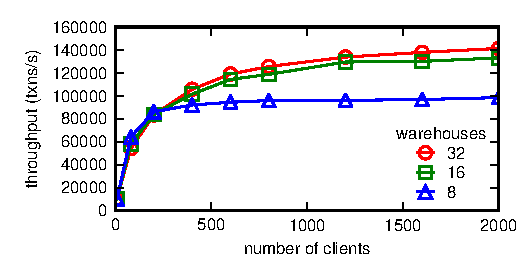
\includegraphics[width=\columnwidth]{figs/wh_thru.pdf}\vspace{-1em}
%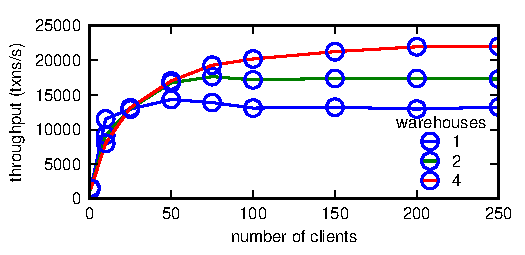
\includegraphics[width=\columnwidth]{figs/wh_thru_single.pdf}
\caption{TPC-C New-Order throughput across eight servers.}
\label{fig:clients}
\end{figure}

\begin{figure}
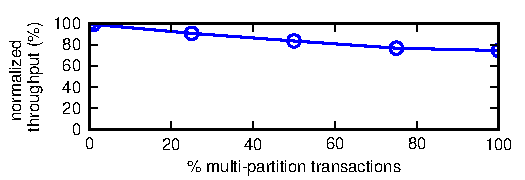
\includegraphics[width=\columnwidth]{figs/pct_thru.pdf}\vspace{-1em}
\caption{Coordination-free distributed execution of TPC-C New-Order
  (primary cost: CPU overhead due to serialization).}
\label{fig:pct}
\end{figure}

Unsurprisingly, a coordination-avoiding strategy allows linear scaling
(Figure~\ref{fig:scaleout}). On 100 EC2 \texttt{cc2.8xlarge} servers
in three \texttt{us-west} availability zones ($5$ warehouses per
server), we achieve over 1.6 million New-Order transactions per
second. We achieve 89.5\% of perfect scaling from one to 100 machines
and perfect scaling from ten to 100 machines. At peak, each server is
CPU bound due to our admittedly fairly inefficient
implementation. Nonetheless, by avoiding distributed coordination, 
the system scales out. A comparison with a serializable or Snapshot
Isolated system would be unfair, but we are unaware of any other
compliant TPC-C implementation that achieves greater than $500K$
New-Order transactions per second (e.g., Oracle 11G,
Calvin~\cite{calvin}, Silo's non-FastIDs~\cite{silo},
VLL~\cite{abadi-vll}). In contrast, we present these results as a
proof of concept that executing even ``challenging'' workloads like
TPC-C that contain complex integrity constraints are not at odds with
scalability if implemented in a coordination-avoiding manner.

\begin{figure}
\begin{center}
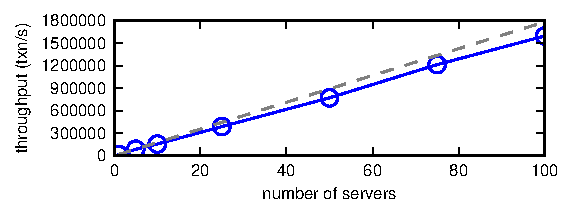
\includegraphics[width=\columnwidth]{figs/thru_scale.pdf}\vspace{-2em}
\end{center}
\caption{Coordination-free distributed execution of TPC-C New-Order is
  linearly scalable (dashed line is perfect scaling).}
\label{fig:scaleout}
\end{figure}

\minihead{Additional transactions} The remaining TPC-C transactions
are are largely uninteresting~\cite{calvin}: all transactions except
Delivery are implementable via a combination of foreign key updates
and commutative counter increment/decrement, and Delivery is easily
implemented (as acknowledged in the benchmark
specification~\cite{tpcc}) as a single-partition transaction. The
TPC-C isolation requirements (reflecting the ANSI SQL specification)
are all achievable via client-side caching~\cite{hat-vldb}.

\subsection{Discussion}

These results begin to quantify the effects of coordination-avoiding
concurrency control. When conflicts cannot be avoided, coordination
(and atomic commitment) can be expensive. However, if considering
\textit{application-level} invariants, databases only have to pay the
price of coordination when required. We were surprised that the
``current industry standard for evaluating the performance of OLTP
systems''~\cite{oltpbench} was so amenable to coordination-free
execution.

We are also aware that TPC-C may be a simplification of real-world
workloads, so for greater variety, we examined the OLTP-Bench
suite~\cite{oltpbench}. We found (and confirmed with an author
of~\cite{oltpbench}) that nine of fourteen remaining (non TPC-C)
benchmarks, the workload transactions did not involve integrity
constraints (e.g., did not modify primary key columns), one
(\texttt{CH-bencCHmark}) matched TPC-C, and two specifications implied
(but did not explicitly state) a requirement for synchronous
coordination due to unique ID assignment (\texttt{AuctionMark}'s
\texttt{new-purchase}, \texttt{SEATS}'s \texttt{NewReservation};
achievable like TPC-C order IDs). The remaining two benchmarks,
\texttt{sibench} and \texttt{smallbank} were specifically designed as
research benchmarks for serializable isolation. The three
``consistency conditions'' in the newer TPC-E benchmark are a subset
of the twelve conditions from TPC-C considered here (all materialized
counters). It is possible (even likely) that these benchmarks are
underspecified, but according to official specifications, TPC-C
contains the most coordination-intensive invariants among the
non-serializable (i.e., all but two academic) benchmarks we
encountered.

Anecdotally, our conversations with end-users have not identified
invariants that are radically different than those we have proposed,
and a simple thought experiment identifying the invariants required
for, say, a social networking site, are fairly simple (e.g., username
uniqueness, foreign key constraints between updates, privacy
settings~\cite{pnuts}). Nonetheless, we view the further study of
real-world invariants to be a necessary area for future
investigation. In the interim, these preliminary results hint at what
is possible with coordination-avoidance as well as the costs of
coordination if \cfreedom is unachievable.


